\section{Design \& Implementation} \label{design}
\subsection{Modulating Acceleration and Deceleration}
Swink discussed different ways to modulate the player avatar movement in the chapter \textit{Response Metrics} \cite{swink}. Inspired by ADSR envelopes (Attack-Decay-Sustain-Release), which are often used in order make an electronic musical instrument mimic the sound of a mechanical instrument \cite{adsr}, he proposed the idea of using velocity modulation to change the game feel. By altering the attack and release phase (or, acceleration and deceleration), it is possible to create different game feel, as illustrated by Figures \ref{fig:adsr_stiff} and \ref{fig:adsr_loose}.

%, e.g., the sound of a pipe organ or a guitar string. This is achieved by modulating the amplitude over time.

%Inspired by Swink's discussion about \textit{Response Metrics} \cite{swink}, a 2D platforming game was developed. The game changes two types of parameters between each round: how fast the ball accelerates and how fast it decelerates when moving horizontally. Swink calls these the \textit{attack} and \textit{release} phases, or, the acceleration and deceleration of avatar movement. Hence, the velocity of the player's avatar is modulated over time, creating different types of game feel. Figures \ref{fig:adsr_stiff} and \ref{fig:adsr_loose} show two examples of the modulations proposed by Swink.


%According to Swink, when the acceleration or deceleration is very long (e.g., the avatar takes more than 100 milliseconds to be perceived to be moving), the impression of instantaneous response erodes. Even if there are small changes in the velocity, if these cannot be perceived by the player, the game might feel unresponsive \cite{swink}. This is illustrated by Figure \ref{fig:adsr}.

\begin{figure}[htbp]
\centering
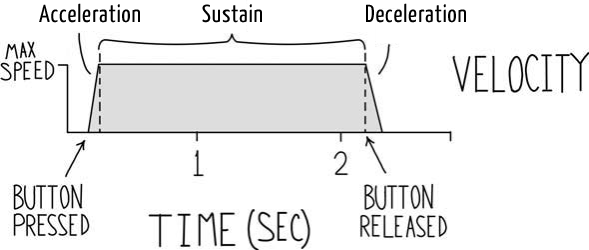
\includegraphics[width=0.30\textwidth]{Pics/adsr_stiff}
\caption{Short acceleration/deceleration gives a responsive, but stiff, feel. Figure inspired by Swink \cite{swink}.}
\label{fig:adsr_stiff}
\end{figure}

\begin{figure}[htbp]
\centering
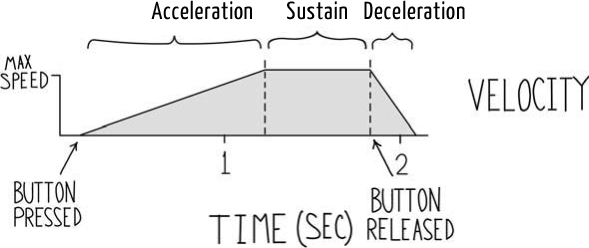
\includegraphics[width=0.30\textwidth]{Pics/adsr_loose}
\caption{Long acceleration gives a loose, but fluid, feel. Figure inspired by Swink \cite{swink}.}
\label{fig:adsr_loose}
\end{figure}

Taking inspiration from Swink, a game was developed with this concept in mind. The game changes two types of parameters between each round: how fast the ball accelerates and how fast it decelerates (when moving horizontally). Hence, the velocity of the player's avatar is modulated over time. This means that when the player presses the movement button, the ball will take a certain amount of time before it reaches its maximum velocity. The same is applied when the player releases the button: the ball will gradually slow down, until it stops.


\begin{figure}[htbp]
\centering
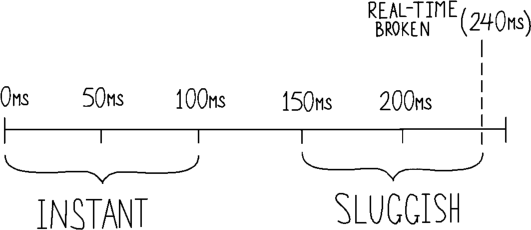
\includegraphics[width=0.30\textwidth]{Pics/response}
\caption{Model of response time and player perception. Figure inspired by Swink \cite{swink}.}
\label{fig:response}
\end{figure}
%Depending on how big a delay there is from the player triggering an event to getting feedback, the game will gradually feel less responsive.

Two intervals were chosen, inspired by Swink's model of player perception and feedback (see Figure \ref{fig:response}). The first interval, \textit{fast}, is between 1 millisecond and 240 milliseconds (staying within the limits of real-time perception). The second interval, \textit{slow}, is from 241 milliseconds to 1500 milliseconds (see Table \ref{tab:time}). For each round in the game, the player is assigned randomly-chosen time values within the two intervals. The reason for choosing random values instead of fixed values is that it isn't perfectly clear at what exact point a game goes from feeling responsive to unresponsive (it's a gradual scale, as shown in Figure \ref{fig:response}). Additionally, the model in Figure \ref{fig:response} depicts the perception of getting discrete feedback, e.g., clicking on a button turns on a light bulb after 50 milliseconds. In the case of avatar movement, there is a continuous stream feedback while the player is holding the movement button, since the avatar is gradually moving forward. However, if the acceleration/deceleration time is very big, the avatar will take some time before it gathers a velocity that can be perceived by the player. In other words, the time values change the total amount of time it takes from when a player presses a button to when the avatar reaches its maximum velocity (or, when releasing the button, reaches a velocity of zero). The acceleration/deceleration is thus scaled depending on the time values, using Equation \ref{eq:erl}.
\begin{equation} \label{eq:erl} %% source: http://www.calculatorsoup.com/calculators/physics/velocity_a_t.php
a = (v - v_0)/t
\end{equation} 
where $a$ is the acceleration/deceleration, $v$ is the target (maximum) velocity, $v_0$ is the initial velocity and $t$ is the time.

%%% This is how to insert a table %%%
\begin{table}[htbp]
\small
\centering
\begin{tabular}{|c|c|}
\hline \textbf{Fast}
& \textbf{Slow}\\\hline
[1 ms - 240 ms]
& [241 ms - 1500 ms]
\\\hline
\end{tabular}
\caption{Time intervals for the acceleration/deceleration.}
\label{tab:time}
\end{table}

The game features other parameters, such as friction, gravity, jump velocity and the aforementioned ghost jump, but only the horizontal ground acceleration and deceleration changed between rounds. The values for these other parameters can be found in APPENDIX A.

The game was developed using the Unity game engine, which allows for exporting to both web and standalone platforms. The game was released for web\footnote{Unity recently made it possible to export to the WebGL platform, but at the time of writing there are bugs and performance issues, so it was chosen to use the standard web player using a browser plug-in.} and Windows. It's a traditional 2D side-scrolling platform game in which players move a small soccer ball from left to right to collect three stars. The game is controlled with the arrow keys and the spacebar.

\subsection{Experimental Design}
The experiment has been designed as a repeated-measures, within-participant design \cite{cunningham}. This means that the participants will be exposed to the stimuli (the changing acceleration and deceleration) multiple times. Additionally, each participant will see all of the available stimuli, thereby acting as their own control group by comparing the different stimuli to each other.

\subsubsection{Latin Squares} \label{latinSection}
There are four possible combinations, as shown in Table \ref{tab:combinations}. One of the strengths with within-participant designs is that it doesn't require as many participants as a between-participant design, since each participant will try all the conditions. However, one disadvantage of within-participant designs is the risk of carry-over effects \cite{experimental1}. This might be due to fatigue (e.g., the participants become bored after having experienced the multiple conditions) or practice (e.g., the participants are better at the end than when they started).

%%% This is how to insert a table %%%
\begin{table}[htbp]
\small
\centering
\begin{tabular}{|c|c|c|}
\hline  & \textbf{Acceleration}
& \textbf{Deceleration}\\\hline
\textbf{Stimulus 1} & Fast (A)
& Fast (A)
\\\hline
\textbf{Stimulus 2} & Slow (B)
& Slow (B)
\\\hline
\textbf{Stimulus 3} & Fast (A)
& Slow (B)
\\\hline
\textbf{Stimulus 4} & Slow (B)
& Fast (A)
\\\hline
\end{tabular}
\caption{Four different combinations.}
\label{tab:combinations}
\end{table}

The order in which the different stimuli is shown can affect the participant's behaviour.  A way to prevent this is to use a counter-balanced design. This method reduces the chances of the order influencing the results \cite{experimental2}. Ideally, since there are four possible conditions (see Table \ref{tab:combinations}), there should be 4x3x2x1 different orders, i.e., 24 orders of treatment. The number of participants must also be a multiple of 24, since there should be an equal number in each group \cite{experimental2}. This was deemed to complex, so instead an incomplete balanced design in the form of Latin squares have been used (see Table \ref{table:latin}). Even though the order effects aren't eliminated completely, they become balanced. Latin squares are arranged in rows and columns such that each of the stimuli conditions only occur once in each row and column. For experiments with an even number of conditions, the first row of a Latin square follows the formula $1, 2, n, 3, n-1, 4, n-2...$, where $n$ is the number of conditions. For subsequent rows, 1 is added to the previous and returning to 1 after $n$ \cite{experimental2}. Using this method, only four different orders are needed. This means that the first player will experience order 1, the second player order 2, etc.

%%% This is how to insert a table %%%
\begin{table}[htbp]
\scriptsize
\centering
\begin{tabular}{|c|c|c|c|c|}
\hline
 & \textbf{Stimulus 1} & \textbf{Stimulus 2} & \textbf{Stimulus 3} & \textbf{Stimulus 4}\\
 \hline
\textbf{Seq. 1} & AA & BB & BA & AB\\
\hline
\textbf{Seq. 2} & BB & AB & AA & BA\\
\hline
\textbf{Seq. 3} & AB & BA & BB & AA\\
\hline
\textbf{Seq. 4} & BA & AA & AB & BB\\
\hline
\end{tabular}
\caption{Latin square showing the four possible sequences. The first letter is the acceleration, the second letter is the deceleration. A means fast and B means slow.}
\label{table:latin}
\end{table}

%\subsection{The Game Itself}

\subsubsection{Structure of the Game}
Taking inspiration from Section \ref{marioLevel}, a questionnaire was built into the game. Before the game begins, players are asked to fill in basic demographical information. After this, players are presented with two examples of the extreme conditions (very fast and very slow acceleration/deceleration). This is called \textit{anchoring} \cite{cunningham} and gives players an idea of what to expect in the game, without explicitly telling them what the examples consists of. Afterwards, the game starts and and players are asked to find and collect three stars. The purpose of the stars is to ensure that players move/jump around enough in order to experience the feel of controlling the ball. The stars have been placed in the beginning, middle and end of the level, so players have to experience the whole level each time. The level consists of traditional platforming elements, as well as obstacles in the form of a few moving enemies and spikes. Figure \ref{fig:level} shows an overview of the game's level.

\begin{figure*}[htbp]
\centering
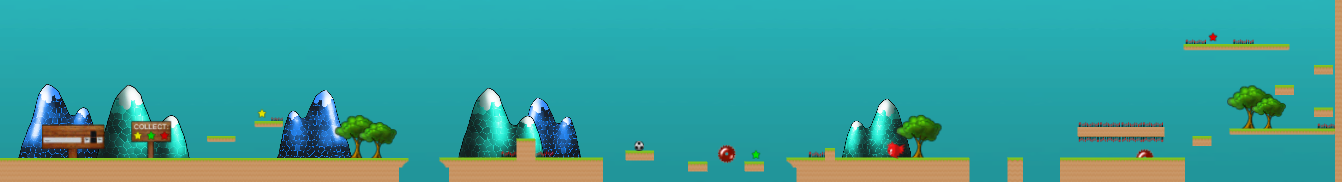
\includegraphics[width=1\textwidth]{Pics/levelStructure}
\caption{Participants play the same level four times.}
\label{fig:level}
\end{figure*}

Each time players collect three stars, the game is paused and a questionnaire is shown (see Figure \ref{fig:questionnaire}). The questionnaire consists of three sets of questions. The first asks players to try and describe the feeling of controlling the ball on the ground and in the air. Inspired by Section {colour}, it is stressed that the chosen word(s) should be something that the player would use to describe the feeling to e.g. a friend. As in Section \ref{colour}, there are no restriction on what types of words players use. In the input box, a few examples are shown to give players an idea of what could be used. These words are chosen randomly and includes adjectives such as `rigid', `reduced', `slow', `dry', `mechanical' and `juicy'. Players are asked to describe the feeling both on the ground and in air. Even though only horizontal movement is changed in the form of the acceleration and deceleration (both apply on ground and in air), there is a possibility that players perceive the game feel differently on ground and in air. Instead of trying to describe both at the same time, players are shown two input fields.

After describing the game feel with the players' own words, a new set of questions are shown. Here, players are asked to rate the game feel on a 7-point Likert scale. Taking inspiration from Swink's book \cite{swink}, players rate the game feeling on how `twitchy', `fluid', `stiff', `floaty' and `responsive' they felt the controls were. Lastly, players are asked about how \textit{enjoyable}, \textit{difficult} and \textit{frustrating} it was to control the ball, as well as \textit{how much they liked} the control of the ball. In case players forgot how it felt to control the ball, they can always click on the \textit{Resume Playing} button and refresh their memories.

\begin{figure*}[htbp]
\centering
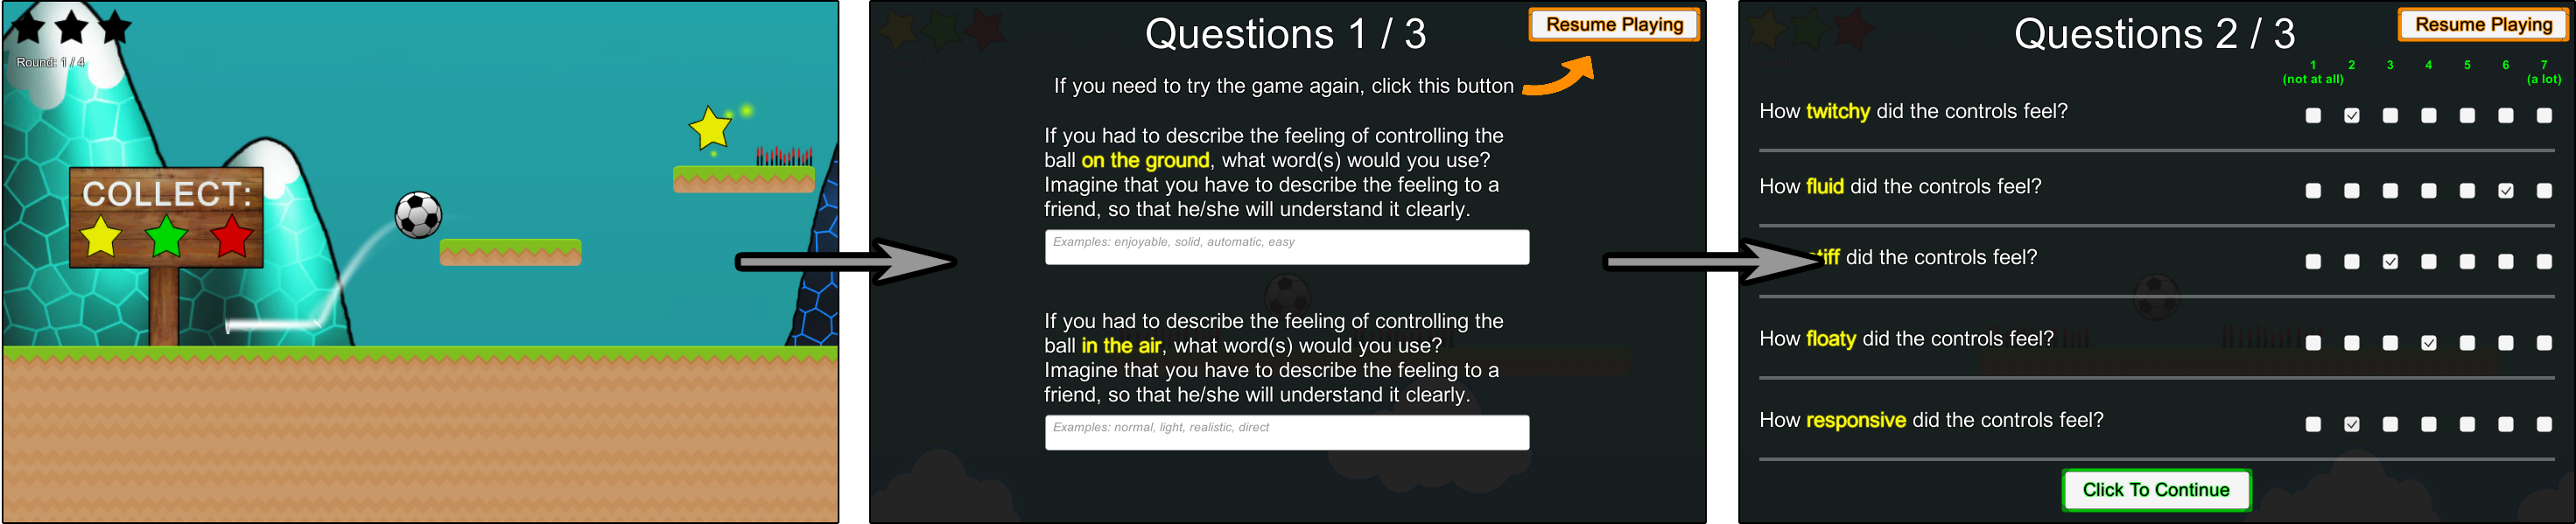
\includegraphics[width=0.95\textwidth]{Pics/game_phases}
\caption{When the player has collected three stars, the game pauses and shows a questionnaire.}
\label{fig:questionnaire}
\end{figure*}

\subsection{Gathering Data}
The game was uploaded to a server and shared on social media websites and gaming forums over the span of one week. A landing page was created where participants could choose to either play the game in their browsers or download a standalone build\footnote{The game is available here: \\ \url{http://tunnelvisiongames.com/g/GameFeel.html}.}. Additionally, Bitly \cite{bitly} was used to keep track of where the link was shared.

Whenever a player completed a round (collecting three stars and answering the questionnaire), data was  sent to an MySQL database. The data entry includes demographical information (age, gender, region, previous experience with games), parameter information (acceleration and deceleration times) and player descriptions (how players describe the game feel, and how they rate the game feel on the pre-defined scales). Target platform (web player or Windows player), player death count, average framerate and time spent on the level were also stored.

To ensure the order in the Latin square (see Section \ref{latinSection}), players were assigned a number between 1 and 4 when starting the game. This number corresponds to the sequences in Table \ref{table:latin}. This was achieved by taking modulus 4 of the total amount of players having completed the test and adding one to it. For instance, if 26 participants had played the game before entering, the next player would be assigned the sequence number (26 \% 4) + 1 = 3.